\documentclass[12pt,letterpaper]{article}
\usepackage{amsmath}
\usepackage{amsfonts}
\usepackage{amsthm}
\usepackage{cancel}
\usepackage[margin=1in]{geometry}
\usepackage{titling}
\usepackage{graphicx}

\setlength{\droptitle}{-10ex}

\preauthor{\begin{flushright}\large \lineskip 0.5em}
\postauthor{\par\end{flushright}}
\predate{\begin{flushright}\large}
\postdate{\par\end{flushright}}

\title{ECS 170 Homework 3\vspace{-2ex}}
\author{Hardy Jones\\
        999397426\\
        Professor Davidson\vspace{-2ex}}
\date{Winter 2014}

\begin{document}
  \maketitle

  \begin{enumerate}
    \item
      We discussed the $\alpha-\beta$ pruning technique for improving the runtime of the minimax algorithm.
      Given a game tree with maximum depth $m$, branching factor $b$, and minimum depth of an optimal state $d$:

      \begin{enumerate}
        \item What is the worst case runtime?

          The worst case runtime is $O(b^m)$.
        \item What is the best case runtime?

          The best case runtime is $O(b^\frac{m}{2})$
        \item Under what condition can we achieve best case runtime?

          The best case can be achieved if we examine the best successors first.
      \end{enumerate}
    \item
      Consider the following min-max game tree.

      \begin{enumerate}
        \item
          Execute $\alpha-\beta$ pruning on the example.
          First, write the minimax value at each node.
          Then cross out the branches that get pruned by $\alpha-\beta$ pruning.
          If a branch does get pruned, circle the nodes under that branch that you had to explore in order to decide to prune the branch.

          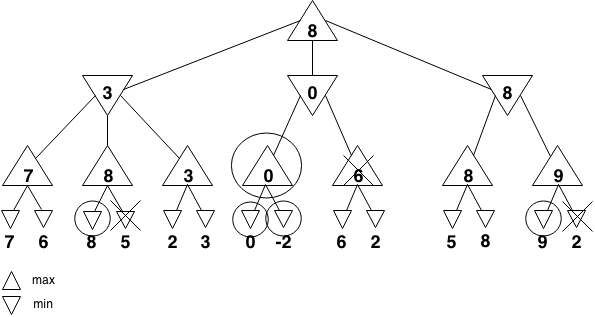
\includegraphics[width=5.5in]{minimax_circled.png}
      \end{enumerate}
  \end{enumerate}
\end{document}
